\documentclass[twoside]{book}

% Packages required by doxygen
\usepackage{fixltx2e}
\usepackage{calc}
\usepackage{doxygen}
\usepackage[export]{adjustbox} % also loads graphicx
\usepackage{graphicx}
\usepackage[utf8]{inputenc}
\usepackage{makeidx}
\usepackage{multicol}
\usepackage{multirow}
\PassOptionsToPackage{warn}{textcomp}
\usepackage{textcomp}
\usepackage[nointegrals]{wasysym}
\usepackage[table]{xcolor}

% Font selection
\usepackage[T1]{fontenc}
\usepackage[scaled=.90]{helvet}
\usepackage{courier}
\usepackage{amssymb}
\usepackage{sectsty}
\renewcommand{\familydefault}{\sfdefault}
\allsectionsfont{%
  \fontseries{bc}\selectfont%
  \color{darkgray}%
}
\renewcommand{\DoxyLabelFont}{%
  \fontseries{bc}\selectfont%
  \color{darkgray}%
}
\newcommand{\+}{\discretionary{\mbox{\scriptsize$\hookleftarrow$}}{}{}}

% Page & text layout
\usepackage{geometry}
\geometry{%
  a4paper,%
  top=2.5cm,%
  bottom=2.5cm,%
  left=2.5cm,%
  right=2.5cm%
}
\tolerance=750
\hfuzz=15pt
\hbadness=750
\setlength{\emergencystretch}{15pt}
\setlength{\parindent}{0cm}
\setlength{\parskip}{3ex plus 2ex minus 2ex}
\makeatletter
\renewcommand{\paragraph}{%
  \@startsection{paragraph}{4}{0ex}{-1.0ex}{1.0ex}{%
    \normalfont\normalsize\bfseries\SS@parafont%
  }%
}
\renewcommand{\subparagraph}{%
  \@startsection{subparagraph}{5}{0ex}{-1.0ex}{1.0ex}{%
    \normalfont\normalsize\bfseries\SS@subparafont%
  }%
}
\makeatother

% Headers & footers
\usepackage{fancyhdr}
\pagestyle{fancyplain}
\fancyhead[LE]{\fancyplain{}{\bfseries\thepage}}
\fancyhead[CE]{\fancyplain{}{}}
\fancyhead[RE]{\fancyplain{}{\bfseries\leftmark}}
\fancyhead[LO]{\fancyplain{}{\bfseries\rightmark}}
\fancyhead[CO]{\fancyplain{}{}}
\fancyhead[RO]{\fancyplain{}{\bfseries\thepage}}
\fancyfoot[LE]{\fancyplain{}{}}
\fancyfoot[CE]{\fancyplain{}{}}
\fancyfoot[RE]{\fancyplain{}{\bfseries\scriptsize Generated by Doxygen }}
\fancyfoot[LO]{\fancyplain{}{\bfseries\scriptsize Generated by Doxygen }}
\fancyfoot[CO]{\fancyplain{}{}}
\fancyfoot[RO]{\fancyplain{}{}}
\renewcommand{\footrulewidth}{0.4pt}
\renewcommand{\chaptermark}[1]{%
  \markboth{#1}{}%
}
\renewcommand{\sectionmark}[1]{%
  \markright{\thesection\ #1}%
}

% Indices & bibliography
\usepackage{natbib}
\usepackage[titles]{tocloft}
\setcounter{tocdepth}{3}
\setcounter{secnumdepth}{5}
\makeindex

% Hyperlinks (required, but should be loaded last)
\usepackage{ifpdf}
\ifpdf
  \usepackage[pdftex,pagebackref=true]{hyperref}
\else
  \usepackage[ps2pdf,pagebackref=true]{hyperref}
\fi
\hypersetup{%
  colorlinks=true,%
  linkcolor=blue,%
  citecolor=blue,%
  unicode%
}

% Custom commands
\newcommand{\clearemptydoublepage}{%
  \newpage{\pagestyle{empty}\cleardoublepage}%
}

\usepackage{caption}
\captionsetup{labelsep=space,justification=centering,font={bf},singlelinecheck=off,skip=4pt,position=top}

%===== C O N T E N T S =====

\begin{document}

% Titlepage & ToC
\hypersetup{pageanchor=false,
             bookmarksnumbered=true,
             pdfencoding=unicode
            }
\pagenumbering{alph}
\begin{titlepage}
\vspace*{7cm}
\begin{center}%
{\Large Doxygen Demo App \\[1ex]\large 1 }\\
\vspace*{1cm}
{\large Generated by Doxygen 1.8.14}\\
\end{center}
\end{titlepage}
\clearemptydoublepage
\pagenumbering{roman}
\tableofcontents
\clearemptydoublepage
\pagenumbering{arabic}
\hypersetup{pageanchor=true}

%--- Begin generated contents ---
\chapter{Namespace Index}
\section{Packages}
Here are the packages with brief descriptions (if available)\+:\begin{DoxyCompactList}
\item\contentsline{section}{\mbox{\hyperlink{namespace_doxygen_demo_application}{Doxygen\+Demo\+Application}} }{\pageref{namespace_doxygen_demo_application}}{}
\item\contentsline{section}{\mbox{\hyperlink{namespace_doxygen_demo_application_1_1_controllers}{Doxygen\+Demo\+Application.\+Controllers}} }{\pageref{namespace_doxygen_demo_application_1_1_controllers}}{}
\item\contentsline{section}{\mbox{\hyperlink{namespace_doxygen_demo_application_1_1_tests}{Doxygen\+Demo\+Application.\+Tests}} }{\pageref{namespace_doxygen_demo_application_1_1_tests}}{}
\item\contentsline{section}{\mbox{\hyperlink{namespace_doxygen_demo_application_1_1_tests_1_1_controllers}{Doxygen\+Demo\+Application.\+Tests.\+Controllers}} }{\pageref{namespace_doxygen_demo_application_1_1_tests_1_1_controllers}}{}
\end{DoxyCompactList}

\chapter{Hierarchical Index}
\section{Class Hierarchy}
This inheritance list is sorted roughly, but not completely, alphabetically\+:\begin{DoxyCompactList}
\item \contentsline{section}{Doxygen\+Demo\+Application.\+Bundle\+Config}{\pageref{class_doxygen_demo_application_1_1_bundle_config}}{}
\item Controller\begin{DoxyCompactList}
\item \contentsline{section}{Doxygen\+Demo\+Application.\+Controllers.\+Home\+Controller}{\pageref{class_doxygen_demo_application_1_1_controllers_1_1_home_controller}}{}
\end{DoxyCompactList}
\item \contentsline{section}{Doxygen\+Demo\+Application.\+Filter\+Config}{\pageref{class_doxygen_demo_application_1_1_filter_config}}{}
\item \contentsline{section}{Doxygen\+Demo\+Application.\+Tests.\+Controllers.\+Home\+Controller\+Test}{\pageref{class_doxygen_demo_application_1_1_tests_1_1_controllers_1_1_home_controller_test}}{}
\item Http\+Application\begin{DoxyCompactList}
\item \contentsline{section}{Doxygen\+Demo\+Application.\+Mvc\+Application}{\pageref{class_doxygen_demo_application_1_1_mvc_application}}{}
\end{DoxyCompactList}
\item \contentsline{section}{Doxygen\+Demo\+Application.\+Route\+Config}{\pageref{class_doxygen_demo_application_1_1_route_config}}{}
\end{DoxyCompactList}

\chapter{Class Index}
\section{Class List}
Here are the classes, structs, unions and interfaces with brief descriptions\+:\begin{DoxyCompactList}
\item\contentsline{section}{\mbox{\hyperlink{class_doxygen_demo_application_1_1_bundle_config}{Doxygen\+Demo\+Application.\+Bundle\+Config}} }{\pageref{class_doxygen_demo_application_1_1_bundle_config}}{}
\item\contentsline{section}{\mbox{\hyperlink{class_doxygen_demo_application_1_1_filter_config}{Doxygen\+Demo\+Application.\+Filter\+Config}} }{\pageref{class_doxygen_demo_application_1_1_filter_config}}{}
\item\contentsline{section}{\mbox{\hyperlink{class_doxygen_demo_application_1_1_controllers_1_1_home_controller}{Doxygen\+Demo\+Application.\+Controllers.\+Home\+Controller}} }{\pageref{class_doxygen_demo_application_1_1_controllers_1_1_home_controller}}{}
\item\contentsline{section}{\mbox{\hyperlink{class_doxygen_demo_application_1_1_tests_1_1_controllers_1_1_home_controller_test}{Doxygen\+Demo\+Application.\+Tests.\+Controllers.\+Home\+Controller\+Test}} }{\pageref{class_doxygen_demo_application_1_1_tests_1_1_controllers_1_1_home_controller_test}}{}
\item\contentsline{section}{\mbox{\hyperlink{class_doxygen_demo_application_1_1_mvc_application}{Doxygen\+Demo\+Application.\+Mvc\+Application}} }{\pageref{class_doxygen_demo_application_1_1_mvc_application}}{}
\item\contentsline{section}{\mbox{\hyperlink{class_doxygen_demo_application_1_1_route_config}{Doxygen\+Demo\+Application.\+Route\+Config}} }{\pageref{class_doxygen_demo_application_1_1_route_config}}{}
\end{DoxyCompactList}

\chapter{File Index}
\section{File List}
Here is a list of all files with brief descriptions\+:\begin{DoxyCompactList}
\item\contentsline{section}{Doxygen\+Demo\+Application.\+Tests/\+Controllers/\mbox{\hyperlink{_home_controller_test_8cs}{Home\+Controller\+Test.\+cs}} }{\pageref{_home_controller_test_8cs}}{}
\item\contentsline{section}{Doxygen\+Demo\+Application.\+Tests/obj/\+Debug/\mbox{\hyperlink{_tests_2obj_2_debug_2_temporary_generated_file__036_c0_b5_b-1481-4323-8_d20-8_f5_a_d_c_b23_d92_8cs}{Temporary\+Generated\+File\+\_\+036\+C0\+B5\+B-\/1481-\/4323-\/8\+D20-\/8\+F5\+A\+D\+C\+B23\+D92.\+cs}} }{\pageref{_tests_2obj_2_debug_2_temporary_generated_file__036_c0_b5_b-1481-4323-8_d20-8_f5_a_d_c_b23_d92_8cs}}{}
\item\contentsline{section}{Doxygen\+Demo\+Application.\+Tests/obj/\+Debug/\mbox{\hyperlink{_tests_2obj_2_debug_2_temporary_generated_file__5937a670-0e60-4077-877b-f7221da3dda1_8cs}{Temporary\+Generated\+File\+\_\+5937a670-\/0e60-\/4077-\/877b-\/f7221da3dda1.\+cs}} }{\pageref{_tests_2obj_2_debug_2_temporary_generated_file__5937a670-0e60-4077-877b-f7221da3dda1_8cs}}{}
\item\contentsline{section}{Doxygen\+Demo\+Application.\+Tests/obj/\+Debug/\mbox{\hyperlink{_tests_2obj_2_debug_2_temporary_generated_file___e7_a71_f73-0_f8_d-4_b9_b-_b56_e-8_e70_b10_b_c5_d3_8cs}{Temporary\+Generated\+File\+\_\+\+E7\+A71\+F73-\/0\+F8\+D-\/4\+B9\+B-\/\+B56\+E-\/8\+E70\+B10\+B\+C5\+D3.\+cs}} }{\pageref{_tests_2obj_2_debug_2_temporary_generated_file___e7_a71_f73-0_f8_d-4_b9_b-_b56_e-8_e70_b10_b_c5_d3_8cs}}{}
\item\contentsline{section}{Doxygen\+Demo\+Application.\+Tests/\+Properties/\mbox{\hyperlink{_tests_2_properties_2_assembly_info_8cs}{Assembly\+Info.\+cs}} }{\pageref{_tests_2_properties_2_assembly_info_8cs}}{}
\item\contentsline{section}{Doxygen\+Demo\+Application/\mbox{\hyperlink{_global_8asax_8cs}{Global.\+asax.\+cs}} }{\pageref{_global_8asax_8cs}}{}
\item\contentsline{section}{Doxygen\+Demo\+Application/\+App\+\_\+\+Start/\mbox{\hyperlink{_bundle_config_8cs}{Bundle\+Config.\+cs}} }{\pageref{_bundle_config_8cs}}{}
\item\contentsline{section}{Doxygen\+Demo\+Application/\+App\+\_\+\+Start/\mbox{\hyperlink{_filter_config_8cs}{Filter\+Config.\+cs}} }{\pageref{_filter_config_8cs}}{}
\item\contentsline{section}{Doxygen\+Demo\+Application/\+App\+\_\+\+Start/\mbox{\hyperlink{_route_config_8cs}{Route\+Config.\+cs}} }{\pageref{_route_config_8cs}}{}
\item\contentsline{section}{Doxygen\+Demo\+Application/\+Controllers/\mbox{\hyperlink{_home_controller_8cs}{Home\+Controller.\+cs}} }{\pageref{_home_controller_8cs}}{}
\item\contentsline{section}{Doxygen\+Demo\+Application/obj/\+Debug/\mbox{\hyperlink{obj_2_debug_2_temporary_generated_file__036_c0_b5_b-1481-4323-8_d20-8_f5_a_d_c_b23_d92_8cs}{Temporary\+Generated\+File\+\_\+036\+C0\+B5\+B-\/1481-\/4323-\/8\+D20-\/8\+F5\+A\+D\+C\+B23\+D92.\+cs}} }{\pageref{obj_2_debug_2_temporary_generated_file__036_c0_b5_b-1481-4323-8_d20-8_f5_a_d_c_b23_d92_8cs}}{}
\item\contentsline{section}{Doxygen\+Demo\+Application/obj/\+Debug/\mbox{\hyperlink{obj_2_debug_2_temporary_generated_file__5937a670-0e60-4077-877b-f7221da3dda1_8cs}{Temporary\+Generated\+File\+\_\+5937a670-\/0e60-\/4077-\/877b-\/f7221da3dda1.\+cs}} }{\pageref{obj_2_debug_2_temporary_generated_file__5937a670-0e60-4077-877b-f7221da3dda1_8cs}}{}
\item\contentsline{section}{Doxygen\+Demo\+Application/obj/\+Debug/\mbox{\hyperlink{obj_2_debug_2_temporary_generated_file___e7_a71_f73-0_f8_d-4_b9_b-_b56_e-8_e70_b10_b_c5_d3_8cs}{Temporary\+Generated\+File\+\_\+\+E7\+A71\+F73-\/0\+F8\+D-\/4\+B9\+B-\/\+B56\+E-\/8\+E70\+B10\+B\+C5\+D3.\+cs}} }{\pageref{obj_2_debug_2_temporary_generated_file___e7_a71_f73-0_f8_d-4_b9_b-_b56_e-8_e70_b10_b_c5_d3_8cs}}{}
\item\contentsline{section}{Doxygen\+Demo\+Application/\+Properties/\mbox{\hyperlink{_properties_2_assembly_info_8cs}{Assembly\+Info.\+cs}} }{\pageref{_properties_2_assembly_info_8cs}}{}
\end{DoxyCompactList}

\chapter{Namespace Documentation}
\hypertarget{namespace_doxygen_demo_application}{}\section{Doxygen\+Demo\+Application Namespace Reference}
\label{namespace_doxygen_demo_application}\index{Doxygen\+Demo\+Application@{Doxygen\+Demo\+Application}}
\subsection*{Namespaces}
\begin{DoxyCompactItemize}
\item 
namespace \mbox{\hyperlink{namespace_doxygen_demo_application_1_1_controllers}{Controllers}}
\item 
namespace \mbox{\hyperlink{namespace_doxygen_demo_application_1_1_tests}{Tests}}
\end{DoxyCompactItemize}
\subsection*{Classes}
\begin{DoxyCompactItemize}
\item 
class \mbox{\hyperlink{class_doxygen_demo_application_1_1_bundle_config}{Bundle\+Config}}
\item 
class \mbox{\hyperlink{class_doxygen_demo_application_1_1_filter_config}{Filter\+Config}}
\item 
class \mbox{\hyperlink{class_doxygen_demo_application_1_1_mvc_application}{Mvc\+Application}}
\item 
class \mbox{\hyperlink{class_doxygen_demo_application_1_1_route_config}{Route\+Config}}
\end{DoxyCompactItemize}

\hypertarget{namespace_doxygen_demo_application_1_1_controllers}{}\section{Doxygen\+Demo\+Application.\+Controllers Namespace Reference}
\label{namespace_doxygen_demo_application_1_1_controllers}\index{Doxygen\+Demo\+Application.\+Controllers@{Doxygen\+Demo\+Application.\+Controllers}}
\subsection*{Classes}
\begin{DoxyCompactItemize}
\item 
class \mbox{\hyperlink{class_doxygen_demo_application_1_1_controllers_1_1_home_controller}{Home\+Controller}}
\end{DoxyCompactItemize}

\hypertarget{namespace_doxygen_demo_application_1_1_tests}{}\section{Doxygen\+Demo\+Application.\+Tests Namespace Reference}
\label{namespace_doxygen_demo_application_1_1_tests}\index{Doxygen\+Demo\+Application.\+Tests@{Doxygen\+Demo\+Application.\+Tests}}
\subsection*{Namespaces}
\begin{DoxyCompactItemize}
\item 
namespace \mbox{\hyperlink{namespace_doxygen_demo_application_1_1_tests_1_1_controllers}{Controllers}}
\end{DoxyCompactItemize}

\hypertarget{namespace_doxygen_demo_application_1_1_tests_1_1_controllers}{}\section{Doxygen\+Demo\+Application.\+Tests.\+Controllers Namespace Reference}
\label{namespace_doxygen_demo_application_1_1_tests_1_1_controllers}\index{Doxygen\+Demo\+Application.\+Tests.\+Controllers@{Doxygen\+Demo\+Application.\+Tests.\+Controllers}}
\subsection*{Classes}
\begin{DoxyCompactItemize}
\item 
class \mbox{\hyperlink{class_doxygen_demo_application_1_1_tests_1_1_controllers_1_1_home_controller_test}{Home\+Controller\+Test}}
\end{DoxyCompactItemize}

\chapter{Class Documentation}
\hypertarget{class_doxygen_demo_application_1_1_bundle_config}{}\section{Doxygen\+Demo\+Application.\+Bundle\+Config Class Reference}
\label{class_doxygen_demo_application_1_1_bundle_config}\index{Doxygen\+Demo\+Application.\+Bundle\+Config@{Doxygen\+Demo\+Application.\+Bundle\+Config}}
\subsection*{Static Public Member Functions}
\begin{DoxyCompactItemize}
\item 
static void \mbox{\hyperlink{class_doxygen_demo_application_1_1_bundle_config_aaf64b5e04c989cfd414fc1c2b4e05981}{Register\+Bundles}} (Bundle\+Collection bundles)
\end{DoxyCompactItemize}


\subsection{Detailed Description}


Definition at line 6 of file Bundle\+Config.\+cs.



\subsection{Member Function Documentation}
\mbox{\Hypertarget{class_doxygen_demo_application_1_1_bundle_config_aaf64b5e04c989cfd414fc1c2b4e05981}\label{class_doxygen_demo_application_1_1_bundle_config_aaf64b5e04c989cfd414fc1c2b4e05981}} 
\index{Doxygen\+Demo\+Application\+::\+Bundle\+Config@{Doxygen\+Demo\+Application\+::\+Bundle\+Config}!Register\+Bundles@{Register\+Bundles}}
\index{Register\+Bundles@{Register\+Bundles}!Doxygen\+Demo\+Application\+::\+Bundle\+Config@{Doxygen\+Demo\+Application\+::\+Bundle\+Config}}
\subsubsection{\texorpdfstring{Register\+Bundles()}{RegisterBundles()}}
{\footnotesize\ttfamily static void Doxygen\+Demo\+Application.\+Bundle\+Config.\+Register\+Bundles (\begin{DoxyParamCaption}\item[{Bundle\+Collection}]{bundles }\end{DoxyParamCaption})\hspace{0.3cm}{\ttfamily [static]}}



Definition at line 9 of file Bundle\+Config.\+cs.



The documentation for this class was generated from the following file\+:\begin{DoxyCompactItemize}
\item 
Doxygen\+Demo\+Application/\+App\+\_\+\+Start/\mbox{\hyperlink{_bundle_config_8cs}{Bundle\+Config.\+cs}}\end{DoxyCompactItemize}

\hypertarget{class_doxygen_demo_application_1_1_filter_config}{}\section{Doxygen\+Demo\+Application.\+Filter\+Config Class Reference}
\label{class_doxygen_demo_application_1_1_filter_config}\index{Doxygen\+Demo\+Application.\+Filter\+Config@{Doxygen\+Demo\+Application.\+Filter\+Config}}
\subsection*{Static Public Member Functions}
\begin{DoxyCompactItemize}
\item 
static void \mbox{\hyperlink{class_doxygen_demo_application_1_1_filter_config_a75ebe17224ce52689211f60390e29e02}{Register\+Global\+Filters}} (Global\+Filter\+Collection filters)
\end{DoxyCompactItemize}


\subsection{Detailed Description}


Definition at line 6 of file Filter\+Config.\+cs.



\subsection{Member Function Documentation}
\mbox{\Hypertarget{class_doxygen_demo_application_1_1_filter_config_a75ebe17224ce52689211f60390e29e02}\label{class_doxygen_demo_application_1_1_filter_config_a75ebe17224ce52689211f60390e29e02}} 
\index{Doxygen\+Demo\+Application\+::\+Filter\+Config@{Doxygen\+Demo\+Application\+::\+Filter\+Config}!Register\+Global\+Filters@{Register\+Global\+Filters}}
\index{Register\+Global\+Filters@{Register\+Global\+Filters}!Doxygen\+Demo\+Application\+::\+Filter\+Config@{Doxygen\+Demo\+Application\+::\+Filter\+Config}}
\subsubsection{\texorpdfstring{Register\+Global\+Filters()}{RegisterGlobalFilters()}}
{\footnotesize\ttfamily static void Doxygen\+Demo\+Application.\+Filter\+Config.\+Register\+Global\+Filters (\begin{DoxyParamCaption}\item[{Global\+Filter\+Collection}]{filters }\end{DoxyParamCaption})\hspace{0.3cm}{\ttfamily [static]}}



Definition at line 8 of file Filter\+Config.\+cs.



The documentation for this class was generated from the following file\+:\begin{DoxyCompactItemize}
\item 
Doxygen\+Demo\+Application/\+App\+\_\+\+Start/\mbox{\hyperlink{_filter_config_8cs}{Filter\+Config.\+cs}}\end{DoxyCompactItemize}

\hypertarget{class_doxygen_demo_application_1_1_controllers_1_1_home_controller}{}\section{Doxygen\+Demo\+Application.\+Controllers.\+Home\+Controller Class Reference}
\label{class_doxygen_demo_application_1_1_controllers_1_1_home_controller}\index{Doxygen\+Demo\+Application.\+Controllers.\+Home\+Controller@{Doxygen\+Demo\+Application.\+Controllers.\+Home\+Controller}}
Inheritance diagram for Doxygen\+Demo\+Application.\+Controllers.\+Home\+Controller\+:\begin{figure}[H]
\begin{center}
\leavevmode
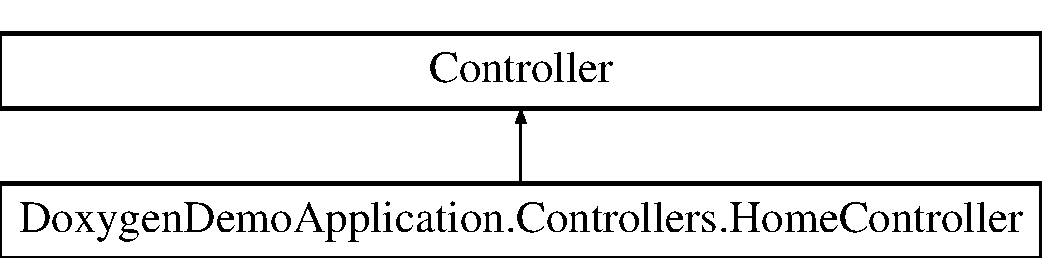
\includegraphics[height=2.000000cm]{class_doxygen_demo_application_1_1_controllers_1_1_home_controller}
\end{center}
\end{figure}
\subsection*{Public Member Functions}
\begin{DoxyCompactItemize}
\item 
Action\+Result \mbox{\hyperlink{class_doxygen_demo_application_1_1_controllers_1_1_home_controller_a9c2494723fb0fbc42a3820972e2318c6}{Index}} ()
\item 
Action\+Result \mbox{\hyperlink{class_doxygen_demo_application_1_1_controllers_1_1_home_controller_a7d6893c8d902a9021181680621912c2a}{About}} ()
\begin{DoxyCompactList}\small\item\em Shows the about page \end{DoxyCompactList}\item 
Action\+Result \mbox{\hyperlink{class_doxygen_demo_application_1_1_controllers_1_1_home_controller_ad2c6cb519deb51651172035e0d4d8e06}{Contact}} ()
\end{DoxyCompactItemize}


\subsection{Detailed Description}


Definition at line 11 of file Home\+Controller.\+cs.



\subsection{Member Function Documentation}
\mbox{\Hypertarget{class_doxygen_demo_application_1_1_controllers_1_1_home_controller_a7d6893c8d902a9021181680621912c2a}\label{class_doxygen_demo_application_1_1_controllers_1_1_home_controller_a7d6893c8d902a9021181680621912c2a}} 
\index{Doxygen\+Demo\+Application\+::\+Controllers\+::\+Home\+Controller@{Doxygen\+Demo\+Application\+::\+Controllers\+::\+Home\+Controller}!About@{About}}
\index{About@{About}!Doxygen\+Demo\+Application\+::\+Controllers\+::\+Home\+Controller@{Doxygen\+Demo\+Application\+::\+Controllers\+::\+Home\+Controller}}
\subsubsection{\texorpdfstring{About()}{About()}}
{\footnotesize\ttfamily Action\+Result Doxygen\+Demo\+Application.\+Controllers.\+Home\+Controller.\+About (\begin{DoxyParamCaption}{ }\end{DoxyParamCaption})}



Shows the about page 

\begin{DoxyReturn}{Returns}

\end{DoxyReturn}


Definition at line 22 of file Home\+Controller.\+cs.

\mbox{\Hypertarget{class_doxygen_demo_application_1_1_controllers_1_1_home_controller_ad2c6cb519deb51651172035e0d4d8e06}\label{class_doxygen_demo_application_1_1_controllers_1_1_home_controller_ad2c6cb519deb51651172035e0d4d8e06}} 
\index{Doxygen\+Demo\+Application\+::\+Controllers\+::\+Home\+Controller@{Doxygen\+Demo\+Application\+::\+Controllers\+::\+Home\+Controller}!Contact@{Contact}}
\index{Contact@{Contact}!Doxygen\+Demo\+Application\+::\+Controllers\+::\+Home\+Controller@{Doxygen\+Demo\+Application\+::\+Controllers\+::\+Home\+Controller}}
\subsubsection{\texorpdfstring{Contact()}{Contact()}}
{\footnotesize\ttfamily Action\+Result Doxygen\+Demo\+Application.\+Controllers.\+Home\+Controller.\+Contact (\begin{DoxyParamCaption}{ }\end{DoxyParamCaption})}



Definition at line 29 of file Home\+Controller.\+cs.

\mbox{\Hypertarget{class_doxygen_demo_application_1_1_controllers_1_1_home_controller_a9c2494723fb0fbc42a3820972e2318c6}\label{class_doxygen_demo_application_1_1_controllers_1_1_home_controller_a9c2494723fb0fbc42a3820972e2318c6}} 
\index{Doxygen\+Demo\+Application\+::\+Controllers\+::\+Home\+Controller@{Doxygen\+Demo\+Application\+::\+Controllers\+::\+Home\+Controller}!Index@{Index}}
\index{Index@{Index}!Doxygen\+Demo\+Application\+::\+Controllers\+::\+Home\+Controller@{Doxygen\+Demo\+Application\+::\+Controllers\+::\+Home\+Controller}}
\subsubsection{\texorpdfstring{Index()}{Index()}}
{\footnotesize\ttfamily Action\+Result Doxygen\+Demo\+Application.\+Controllers.\+Home\+Controller.\+Index (\begin{DoxyParamCaption}{ }\end{DoxyParamCaption})}



Definition at line 13 of file Home\+Controller.\+cs.



The documentation for this class was generated from the following file\+:\begin{DoxyCompactItemize}
\item 
Doxygen\+Demo\+Application/\+Controllers/\mbox{\hyperlink{_home_controller_8cs}{Home\+Controller.\+cs}}\end{DoxyCompactItemize}

\hypertarget{class_doxygen_demo_application_1_1_tests_1_1_controllers_1_1_home_controller_test}{}\section{Doxygen\+Demo\+Application.\+Tests.\+Controllers.\+Home\+Controller\+Test Class Reference}
\label{class_doxygen_demo_application_1_1_tests_1_1_controllers_1_1_home_controller_test}\index{Doxygen\+Demo\+Application.\+Tests.\+Controllers.\+Home\+Controller\+Test@{Doxygen\+Demo\+Application.\+Tests.\+Controllers.\+Home\+Controller\+Test}}
\subsection*{Public Member Functions}
\begin{DoxyCompactItemize}
\item 
void \mbox{\hyperlink{class_doxygen_demo_application_1_1_tests_1_1_controllers_1_1_home_controller_test_a37676ede72810604e3c30e1e5f126ee0}{Index}} ()
\item 
void \mbox{\hyperlink{class_doxygen_demo_application_1_1_tests_1_1_controllers_1_1_home_controller_test_a49e01d0f8582dc219e914dfe71b05a6c}{About}} ()
\item 
void \mbox{\hyperlink{class_doxygen_demo_application_1_1_tests_1_1_controllers_1_1_home_controller_test_af473f3a9c2ca9da46ef0d4c8a4012238}{Contact}} ()
\end{DoxyCompactItemize}


\subsection{Detailed Description}


Definition at line 13 of file Home\+Controller\+Test.\+cs.



\subsection{Member Function Documentation}
\mbox{\Hypertarget{class_doxygen_demo_application_1_1_tests_1_1_controllers_1_1_home_controller_test_a49e01d0f8582dc219e914dfe71b05a6c}\label{class_doxygen_demo_application_1_1_tests_1_1_controllers_1_1_home_controller_test_a49e01d0f8582dc219e914dfe71b05a6c}} 
\index{Doxygen\+Demo\+Application\+::\+Tests\+::\+Controllers\+::\+Home\+Controller\+Test@{Doxygen\+Demo\+Application\+::\+Tests\+::\+Controllers\+::\+Home\+Controller\+Test}!About@{About}}
\index{About@{About}!Doxygen\+Demo\+Application\+::\+Tests\+::\+Controllers\+::\+Home\+Controller\+Test@{Doxygen\+Demo\+Application\+::\+Tests\+::\+Controllers\+::\+Home\+Controller\+Test}}
\subsubsection{\texorpdfstring{About()}{About()}}
{\footnotesize\ttfamily void Doxygen\+Demo\+Application.\+Tests.\+Controllers.\+Home\+Controller\+Test.\+About (\begin{DoxyParamCaption}{ }\end{DoxyParamCaption})}



Definition at line 29 of file Home\+Controller\+Test.\+cs.

\mbox{\Hypertarget{class_doxygen_demo_application_1_1_tests_1_1_controllers_1_1_home_controller_test_af473f3a9c2ca9da46ef0d4c8a4012238}\label{class_doxygen_demo_application_1_1_tests_1_1_controllers_1_1_home_controller_test_af473f3a9c2ca9da46ef0d4c8a4012238}} 
\index{Doxygen\+Demo\+Application\+::\+Tests\+::\+Controllers\+::\+Home\+Controller\+Test@{Doxygen\+Demo\+Application\+::\+Tests\+::\+Controllers\+::\+Home\+Controller\+Test}!Contact@{Contact}}
\index{Contact@{Contact}!Doxygen\+Demo\+Application\+::\+Tests\+::\+Controllers\+::\+Home\+Controller\+Test@{Doxygen\+Demo\+Application\+::\+Tests\+::\+Controllers\+::\+Home\+Controller\+Test}}
\subsubsection{\texorpdfstring{Contact()}{Contact()}}
{\footnotesize\ttfamily void Doxygen\+Demo\+Application.\+Tests.\+Controllers.\+Home\+Controller\+Test.\+Contact (\begin{DoxyParamCaption}{ }\end{DoxyParamCaption})}



Definition at line 42 of file Home\+Controller\+Test.\+cs.

\mbox{\Hypertarget{class_doxygen_demo_application_1_1_tests_1_1_controllers_1_1_home_controller_test_a37676ede72810604e3c30e1e5f126ee0}\label{class_doxygen_demo_application_1_1_tests_1_1_controllers_1_1_home_controller_test_a37676ede72810604e3c30e1e5f126ee0}} 
\index{Doxygen\+Demo\+Application\+::\+Tests\+::\+Controllers\+::\+Home\+Controller\+Test@{Doxygen\+Demo\+Application\+::\+Tests\+::\+Controllers\+::\+Home\+Controller\+Test}!Index@{Index}}
\index{Index@{Index}!Doxygen\+Demo\+Application\+::\+Tests\+::\+Controllers\+::\+Home\+Controller\+Test@{Doxygen\+Demo\+Application\+::\+Tests\+::\+Controllers\+::\+Home\+Controller\+Test}}
\subsubsection{\texorpdfstring{Index()}{Index()}}
{\footnotesize\ttfamily void Doxygen\+Demo\+Application.\+Tests.\+Controllers.\+Home\+Controller\+Test.\+Index (\begin{DoxyParamCaption}{ }\end{DoxyParamCaption})}



Definition at line 16 of file Home\+Controller\+Test.\+cs.



The documentation for this class was generated from the following file\+:\begin{DoxyCompactItemize}
\item 
Doxygen\+Demo\+Application.\+Tests/\+Controllers/\mbox{\hyperlink{_home_controller_test_8cs}{Home\+Controller\+Test.\+cs}}\end{DoxyCompactItemize}

\hypertarget{class_doxygen_demo_application_1_1_mvc_application}{}\section{Doxygen\+Demo\+Application.\+Mvc\+Application Class Reference}
\label{class_doxygen_demo_application_1_1_mvc_application}\index{Doxygen\+Demo\+Application.\+Mvc\+Application@{Doxygen\+Demo\+Application.\+Mvc\+Application}}
Inheritance diagram for Doxygen\+Demo\+Application.\+Mvc\+Application\+:\begin{figure}[H]
\begin{center}
\leavevmode
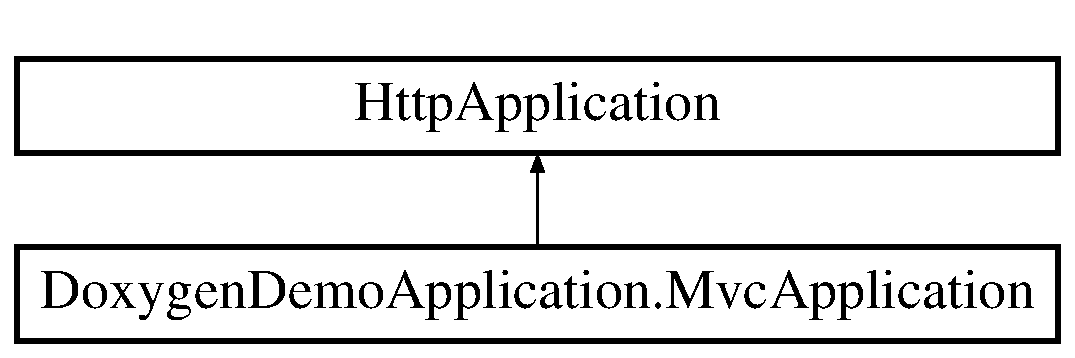
\includegraphics[height=2.000000cm]{class_doxygen_demo_application_1_1_mvc_application}
\end{center}
\end{figure}
\subsection*{Protected Member Functions}
\begin{DoxyCompactItemize}
\item 
void \mbox{\hyperlink{class_doxygen_demo_application_1_1_mvc_application_a65c33faea17a0f68997fc321fdeab52b}{Application\+\_\+\+Start}} ()
\end{DoxyCompactItemize}


\subsection{Detailed Description}


Definition at line 11 of file Global.\+asax.\+cs.



\subsection{Member Function Documentation}
\mbox{\Hypertarget{class_doxygen_demo_application_1_1_mvc_application_a65c33faea17a0f68997fc321fdeab52b}\label{class_doxygen_demo_application_1_1_mvc_application_a65c33faea17a0f68997fc321fdeab52b}} 
\index{Doxygen\+Demo\+Application\+::\+Mvc\+Application@{Doxygen\+Demo\+Application\+::\+Mvc\+Application}!Application\+\_\+\+Start@{Application\+\_\+\+Start}}
\index{Application\+\_\+\+Start@{Application\+\_\+\+Start}!Doxygen\+Demo\+Application\+::\+Mvc\+Application@{Doxygen\+Demo\+Application\+::\+Mvc\+Application}}
\subsubsection{\texorpdfstring{Application\+\_\+\+Start()}{Application\_Start()}}
{\footnotesize\ttfamily void Doxygen\+Demo\+Application.\+Mvc\+Application.\+Application\+\_\+\+Start (\begin{DoxyParamCaption}{ }\end{DoxyParamCaption})\hspace{0.3cm}{\ttfamily [protected]}}



Definition at line 13 of file Global.\+asax.\+cs.



The documentation for this class was generated from the following file\+:\begin{DoxyCompactItemize}
\item 
Doxygen\+Demo\+Application/\mbox{\hyperlink{_global_8asax_8cs}{Global.\+asax.\+cs}}\end{DoxyCompactItemize}

\hypertarget{class_doxygen_demo_application_1_1_route_config}{}\section{Doxygen\+Demo\+Application.\+Route\+Config Class Reference}
\label{class_doxygen_demo_application_1_1_route_config}\index{Doxygen\+Demo\+Application.\+Route\+Config@{Doxygen\+Demo\+Application.\+Route\+Config}}
\subsection*{Static Public Member Functions}
\begin{DoxyCompactItemize}
\item 
static void \mbox{\hyperlink{class_doxygen_demo_application_1_1_route_config_ad8ce309725466085d0a5d34175a0f81b}{Register\+Routes}} (Route\+Collection routes)
\end{DoxyCompactItemize}


\subsection{Detailed Description}


Definition at line 10 of file Route\+Config.\+cs.



\subsection{Member Function Documentation}
\mbox{\Hypertarget{class_doxygen_demo_application_1_1_route_config_ad8ce309725466085d0a5d34175a0f81b}\label{class_doxygen_demo_application_1_1_route_config_ad8ce309725466085d0a5d34175a0f81b}} 
\index{Doxygen\+Demo\+Application\+::\+Route\+Config@{Doxygen\+Demo\+Application\+::\+Route\+Config}!Register\+Routes@{Register\+Routes}}
\index{Register\+Routes@{Register\+Routes}!Doxygen\+Demo\+Application\+::\+Route\+Config@{Doxygen\+Demo\+Application\+::\+Route\+Config}}
\subsubsection{\texorpdfstring{Register\+Routes()}{RegisterRoutes()}}
{\footnotesize\ttfamily static void Doxygen\+Demo\+Application.\+Route\+Config.\+Register\+Routes (\begin{DoxyParamCaption}\item[{Route\+Collection}]{routes }\end{DoxyParamCaption})\hspace{0.3cm}{\ttfamily [static]}}



Definition at line 12 of file Route\+Config.\+cs.



The documentation for this class was generated from the following file\+:\begin{DoxyCompactItemize}
\item 
Doxygen\+Demo\+Application/\+App\+\_\+\+Start/\mbox{\hyperlink{_route_config_8cs}{Route\+Config.\+cs}}\end{DoxyCompactItemize}

\chapter{File Documentation}
\hypertarget{_home_controller_test_8cs}{}\section{Doxygen\+Demo\+Application.\+Tests/\+Controllers/\+Home\+Controller\+Test.cs File Reference}
\label{_home_controller_test_8cs}\index{Doxygen\+Demo\+Application.\+Tests/\+Controllers/\+Home\+Controller\+Test.\+cs@{Doxygen\+Demo\+Application.\+Tests/\+Controllers/\+Home\+Controller\+Test.\+cs}}
\subsection*{Classes}
\begin{DoxyCompactItemize}
\item 
class \mbox{\hyperlink{class_doxygen_demo_application_1_1_tests_1_1_controllers_1_1_home_controller_test}{Doxygen\+Demo\+Application.\+Tests.\+Controllers.\+Home\+Controller\+Test}}
\end{DoxyCompactItemize}
\subsection*{Namespaces}
\begin{DoxyCompactItemize}
\item 
namespace \mbox{\hyperlink{namespace_doxygen_demo_application_1_1_tests_1_1_controllers}{Doxygen\+Demo\+Application.\+Tests.\+Controllers}}
\end{DoxyCompactItemize}

\hypertarget{_bundle_config_8cs}{}\section{Doxygen\+Demo\+Application/\+App\+\_\+\+Start/\+Bundle\+Config.cs File Reference}
\label{_bundle_config_8cs}\index{Doxygen\+Demo\+Application/\+App\+\_\+\+Start/\+Bundle\+Config.\+cs@{Doxygen\+Demo\+Application/\+App\+\_\+\+Start/\+Bundle\+Config.\+cs}}
\subsection*{Classes}
\begin{DoxyCompactItemize}
\item 
class \mbox{\hyperlink{class_doxygen_demo_application_1_1_bundle_config}{Doxygen\+Demo\+Application.\+Bundle\+Config}}
\end{DoxyCompactItemize}
\subsection*{Namespaces}
\begin{DoxyCompactItemize}
\item 
namespace \mbox{\hyperlink{namespace_doxygen_demo_application}{Doxygen\+Demo\+Application}}
\end{DoxyCompactItemize}

\hypertarget{_filter_config_8cs}{}\section{Doxygen\+Demo\+Application/\+App\+\_\+\+Start/\+Filter\+Config.cs File Reference}
\label{_filter_config_8cs}\index{Doxygen\+Demo\+Application/\+App\+\_\+\+Start/\+Filter\+Config.\+cs@{Doxygen\+Demo\+Application/\+App\+\_\+\+Start/\+Filter\+Config.\+cs}}
\subsection*{Classes}
\begin{DoxyCompactItemize}
\item 
class \mbox{\hyperlink{class_doxygen_demo_application_1_1_filter_config}{Doxygen\+Demo\+Application.\+Filter\+Config}}
\end{DoxyCompactItemize}
\subsection*{Namespaces}
\begin{DoxyCompactItemize}
\item 
namespace \mbox{\hyperlink{namespace_doxygen_demo_application}{Doxygen\+Demo\+Application}}
\end{DoxyCompactItemize}

\hypertarget{_route_config_8cs}{}\section{Doxygen\+Demo\+Application/\+App\+\_\+\+Start/\+Route\+Config.cs File Reference}
\label{_route_config_8cs}\index{Doxygen\+Demo\+Application/\+App\+\_\+\+Start/\+Route\+Config.\+cs@{Doxygen\+Demo\+Application/\+App\+\_\+\+Start/\+Route\+Config.\+cs}}
\subsection*{Classes}
\begin{DoxyCompactItemize}
\item 
class \mbox{\hyperlink{class_doxygen_demo_application_1_1_route_config}{Doxygen\+Demo\+Application.\+Route\+Config}}
\end{DoxyCompactItemize}
\subsection*{Namespaces}
\begin{DoxyCompactItemize}
\item 
namespace \mbox{\hyperlink{namespace_doxygen_demo_application}{Doxygen\+Demo\+Application}}
\end{DoxyCompactItemize}

\hypertarget{_home_controller_8cs}{}\section{Doxygen\+Demo\+Application/\+Controllers/\+Home\+Controller.cs File Reference}
\label{_home_controller_8cs}\index{Doxygen\+Demo\+Application/\+Controllers/\+Home\+Controller.\+cs@{Doxygen\+Demo\+Application/\+Controllers/\+Home\+Controller.\+cs}}
\subsection*{Classes}
\begin{DoxyCompactItemize}
\item 
class \mbox{\hyperlink{class_doxygen_demo_application_1_1_controllers_1_1_home_controller}{Doxygen\+Demo\+Application.\+Controllers.\+Home\+Controller}}
\end{DoxyCompactItemize}
\subsection*{Namespaces}
\begin{DoxyCompactItemize}
\item 
namespace \mbox{\hyperlink{namespace_doxygen_demo_application_1_1_controllers}{Doxygen\+Demo\+Application.\+Controllers}}
\end{DoxyCompactItemize}

\hypertarget{_global_8asax_8cs}{}\section{Doxygen\+Demo\+Application/\+Global.asax.\+cs File Reference}
\label{_global_8asax_8cs}\index{Doxygen\+Demo\+Application/\+Global.\+asax.\+cs@{Doxygen\+Demo\+Application/\+Global.\+asax.\+cs}}
\subsection*{Classes}
\begin{DoxyCompactItemize}
\item 
class \mbox{\hyperlink{class_doxygen_demo_application_1_1_mvc_application}{Doxygen\+Demo\+Application.\+Mvc\+Application}}
\end{DoxyCompactItemize}
\subsection*{Namespaces}
\begin{DoxyCompactItemize}
\item 
namespace \mbox{\hyperlink{namespace_doxygen_demo_application}{Doxygen\+Demo\+Application}}
\end{DoxyCompactItemize}

\hypertarget{obj_2_debug_2_temporary_generated_file__036_c0_b5_b-1481-4323-8_d20-8_f5_a_d_c_b23_d92_8cs}{}\section{Doxygen\+Demo\+Application/obj/\+Debug/\+Temporary\+Generated\+File\+\_\+036\+C0\+B5\+B-\/1481-\/4323-\/8\+D20-\/8\+F5\+A\+D\+C\+B23\+D92.cs File Reference}
\label{obj_2_debug_2_temporary_generated_file__036_c0_b5_b-1481-4323-8_d20-8_f5_a_d_c_b23_d92_8cs}\index{Doxygen\+Demo\+Application/obj/\+Debug/\+Temporary\+Generated\+File\+\_\+036\+C0\+B5\+B-\/1481-\/4323-\/8\+D20-\/8\+F5\+A\+D\+C\+B23\+D92.\+cs@{Doxygen\+Demo\+Application/obj/\+Debug/\+Temporary\+Generated\+File\+\_\+036\+C0\+B5\+B-\/1481-\/4323-\/8\+D20-\/8\+F5\+A\+D\+C\+B23\+D92.\+cs}}

\hypertarget{_tests_2obj_2_debug_2_temporary_generated_file__036_c0_b5_b-1481-4323-8_d20-8_f5_a_d_c_b23_d92_8cs}{}\section{Doxygen\+Demo\+Application.\+Tests/obj/\+Debug/\+Temporary\+Generated\+File\+\_\+036\+C0\+B5\+B-\/1481-\/4323-\/8\+D20-\/8\+F5\+A\+D\+C\+B23\+D92.cs File Reference}
\label{_tests_2obj_2_debug_2_temporary_generated_file__036_c0_b5_b-1481-4323-8_d20-8_f5_a_d_c_b23_d92_8cs}\index{Doxygen\+Demo\+Application.\+Tests/obj/\+Debug/\+Temporary\+Generated\+File\+\_\+036\+C0\+B5\+B-\/1481-\/4323-\/8\+D20-\/8\+F5\+A\+D\+C\+B23\+D92.\+cs@{Doxygen\+Demo\+Application.\+Tests/obj/\+Debug/\+Temporary\+Generated\+File\+\_\+036\+C0\+B5\+B-\/1481-\/4323-\/8\+D20-\/8\+F5\+A\+D\+C\+B23\+D92.\+cs}}

\hypertarget{obj_2_debug_2_temporary_generated_file__5937a670-0e60-4077-877b-f7221da3dda1_8cs}{}\section{Doxygen\+Demo\+Application/obj/\+Debug/\+Temporary\+Generated\+File\+\_\+5937a670-\/0e60-\/4077-\/877b-\/f7221da3dda1.cs File Reference}
\label{obj_2_debug_2_temporary_generated_file__5937a670-0e60-4077-877b-f7221da3dda1_8cs}\index{Doxygen\+Demo\+Application/obj/\+Debug/\+Temporary\+Generated\+File\+\_\+5937a670-\/0e60-\/4077-\/877b-\/f7221da3dda1.\+cs@{Doxygen\+Demo\+Application/obj/\+Debug/\+Temporary\+Generated\+File\+\_\+5937a670-\/0e60-\/4077-\/877b-\/f7221da3dda1.\+cs}}

\hypertarget{_tests_2obj_2_debug_2_temporary_generated_file__5937a670-0e60-4077-877b-f7221da3dda1_8cs}{}\section{Doxygen\+Demo\+Application.\+Tests/obj/\+Debug/\+Temporary\+Generated\+File\+\_\+5937a670-\/0e60-\/4077-\/877b-\/f7221da3dda1.cs File Reference}
\label{_tests_2obj_2_debug_2_temporary_generated_file__5937a670-0e60-4077-877b-f7221da3dda1_8cs}\index{Doxygen\+Demo\+Application.\+Tests/obj/\+Debug/\+Temporary\+Generated\+File\+\_\+5937a670-\/0e60-\/4077-\/877b-\/f7221da3dda1.\+cs@{Doxygen\+Demo\+Application.\+Tests/obj/\+Debug/\+Temporary\+Generated\+File\+\_\+5937a670-\/0e60-\/4077-\/877b-\/f7221da3dda1.\+cs}}

\hypertarget{obj_2_debug_2_temporary_generated_file___e7_a71_f73-0_f8_d-4_b9_b-_b56_e-8_e70_b10_b_c5_d3_8cs}{}\section{Doxygen\+Demo\+Application/obj/\+Debug/\+Temporary\+Generated\+File\+\_\+\+E7\+A71\+F73-\/0\+F8\+D-\/4\+B9\+B-\/\+B56\+E-\/8\+E70\+B10\+B\+C5\+D3.cs File Reference}
\label{obj_2_debug_2_temporary_generated_file___e7_a71_f73-0_f8_d-4_b9_b-_b56_e-8_e70_b10_b_c5_d3_8cs}\index{Doxygen\+Demo\+Application/obj/\+Debug/\+Temporary\+Generated\+File\+\_\+\+E7\+A71\+F73-\/0\+F8\+D-\/4\+B9\+B-\/\+B56\+E-\/8\+E70\+B10\+B\+C5\+D3.\+cs@{Doxygen\+Demo\+Application/obj/\+Debug/\+Temporary\+Generated\+File\+\_\+\+E7\+A71\+F73-\/0\+F8\+D-\/4\+B9\+B-\/\+B56\+E-\/8\+E70\+B10\+B\+C5\+D3.\+cs}}

\hypertarget{_tests_2obj_2_debug_2_temporary_generated_file___e7_a71_f73-0_f8_d-4_b9_b-_b56_e-8_e70_b10_b_c5_d3_8cs}{}\section{Doxygen\+Demo\+Application.\+Tests/obj/\+Debug/\+Temporary\+Generated\+File\+\_\+\+E7\+A71\+F73-\/0\+F8\+D-\/4\+B9\+B-\/\+B56\+E-\/8\+E70\+B10\+B\+C5\+D3.cs File Reference}
\label{_tests_2obj_2_debug_2_temporary_generated_file___e7_a71_f73-0_f8_d-4_b9_b-_b56_e-8_e70_b10_b_c5_d3_8cs}\index{Doxygen\+Demo\+Application.\+Tests/obj/\+Debug/\+Temporary\+Generated\+File\+\_\+\+E7\+A71\+F73-\/0\+F8\+D-\/4\+B9\+B-\/\+B56\+E-\/8\+E70\+B10\+B\+C5\+D3.\+cs@{Doxygen\+Demo\+Application.\+Tests/obj/\+Debug/\+Temporary\+Generated\+File\+\_\+\+E7\+A71\+F73-\/0\+F8\+D-\/4\+B9\+B-\/\+B56\+E-\/8\+E70\+B10\+B\+C5\+D3.\+cs}}

\hypertarget{_properties_2_assembly_info_8cs}{}\section{Doxygen\+Demo\+Application/\+Properties/\+Assembly\+Info.cs File Reference}
\label{_properties_2_assembly_info_8cs}\index{Doxygen\+Demo\+Application/\+Properties/\+Assembly\+Info.\+cs@{Doxygen\+Demo\+Application/\+Properties/\+Assembly\+Info.\+cs}}

\hypertarget{_tests_2_properties_2_assembly_info_8cs}{}\section{Doxygen\+Demo\+Application.\+Tests/\+Properties/\+Assembly\+Info.cs File Reference}
\label{_tests_2_properties_2_assembly_info_8cs}\index{Doxygen\+Demo\+Application.\+Tests/\+Properties/\+Assembly\+Info.\+cs@{Doxygen\+Demo\+Application.\+Tests/\+Properties/\+Assembly\+Info.\+cs}}

%--- End generated contents ---

% Index
\backmatter
\newpage
\phantomsection
\clearemptydoublepage
\addcontentsline{toc}{chapter}{Index}
\printindex

\end{document}
